\section {Background: Ecology and Ecosystems}

The credit for coining the word "ökologie" is generally given to Ernst Haeckel who, through a publication in 1866, suggested that this new term should refer to the broad study of nature's economy. This recent coinage does not suggest that ecological thinking only has a history of 160 years. Haeckel likely drew from Linnaeus’ 18th century conception of the “economy of nature” \citep{worster_1977} and the Latin roots of the word literally translate to the "study of the house." If we consider a modern definition of ecology as "... the study of the structure and function of nature, it being understood that mankind is a part of nature" we can trace the lineage of ecological thought back to classical Greece \citep[][p. 3]{odum_1953}. Indeed, if we look to the history of thought on humans and their relationships with nature more broadly, we find the persistence of three general questions \citep{glacken_1967}: \begin{itemize} \item What is nature's influence on man? \item What is man's influence on nature? \item Is there a grand purpose in these relationships? \end{itemize} Stated in a more ecological sense, these questions can be rephrased: \begin{itemize} \item What is the influence of the non-living environment on living organisms? \item What is the influence of living organisms on the non-living environment? \end{itemize} For most of history we have struggled with the first question. Only with the thinking of Darwin did we begin to take it seriously that non-human organisms could be influenced by their surrounding environment. Then with the recent attention to the Anthropocene we have engaged more deeply with the second question. While it is easy to observe relatively small-scale human influences on the environment, we now understand that both human and non-human life alters the environment at planetary scales. The importance of the third question from Glacken is diminishing in academic circles and is generally left to the theologians, yet holistic (dare we say non-scientific) approaches may be just as important to understanding nature as the concepts of stocks and flows of material resources borrowed from economic thought. 

But we digress. It is not really the discipline of ecology with which we concern ourselves, instead the concept of the ecosystem is the object of inquiry. The term ecosystem was introduced less than 100 years ago in a 1935 paper written by Arthur Tansley, an British ecologist frustrated with the use of organismic metaphors to describe biotic communities and their environs (see figure 1). This frustration also extended to applying the metaphor to “human communities as habitually so constituted.” His goal in coining the term was to clarify the notion that the "ecosystem" is an \textit{abstraction} of climate, earth, and life that does not exist outside of human thought \citep{tansley_1935}. An ecosystem is understood as a community of living organisms--the \textit{biocoenosis}: plants, animals, fungi, and so on--and the set of relationships between themselves and with their surrounding non-living environment--the \textit{biotope} \citep{tansley_1935, odum_1953}. Living communities, natural environs, and relationships--ecosystems. According to the Oxford English Dictionary, the term ecology has recently come to refer to simply the relationships found in an ecosystem \citep{oed_2008}. As noted below, one of the difficulties with the information ecosystem metaphor is the confusion of ecologies with ecosystems. For purposes of clarity in this essay the term(s) ecology(ies) will be used in its original sense to refer to the study(ies) of ecosystems and linked socio-natural systems--unless explicitly noted otherwise--not the set of relations found within an ecosystem. 

\subsection{Early ecosystems and evolution}

Evolution, competition, and cooperation have been applied to ecosystem thinking since its inception, although not without difficulties and ideological differences. As originally conceived by Darwin, evolution was largely competitive; individuals from certain species were in constant struggle to claim and maintain their places in nature's economy. His theory of "descent with modification" was developed in the context of Malthusian thinking on human populations in which food resources increase in a linear fashion and population increases in a exponential manner; quickly competitive survival becomes "red in tooth and claw" not only between species, but within the same species \citep{stoddart_1966,tennyson_1849} [note the Tennyson poem originally refers to human relationships!]. 

Well know to history is that this idea of competitive evolution was quickly adopted to explain phenomena in human societies and "the survival of the fittest" was applied to both the relations between humans and between humans and the environment. The first with dire consequences as shown with Hitler's adoption of the notion of \textit{lebensraum}--in which political nation-states are said to "evolve" and claim spaces in the global economy--to justify his crusade to exterminate the Jews, and the second in environmental management rhetoric in which it is our destiny as humans to control and dominate nature \citep{stoddart_1966,worster_1977}. These developments that arose from ideas of competition in Darwin's theory do not preclude ideas of symbiosis or mutualism in the evolution of species, nevertheless. 

At the turn of the 20th century there were thinkers such as Hermann Reinheimer, Petr Kropotkin, and Eugenius Warming who attempted to highlight cooperation and symbiosis as essential strategies for survival in the competitive world \citep{worster_1977}. For example, Petr Kropotkin's work emphasized the cooperative aspects of evolution in both biological and human communities \citep{kropotkin_1902}. While his work was heavily flawed, his thesis leads to current explanations of mutualism in which species co-evolve and rely on one-another to survive. Not coincidental, these thinkers all used the economy of nature metaphor to expand the thinking to include human economic organization in the conversation. No matter that Kropotkin was an anarchist, these ideas were instilled in the work of the later reductionists (see below) and ecology took on the appearance of a subordinate field of economics and econometrics. The ecosystem is understood as a mirror of human economic production and consumption in which the self-reliant competitor is a but a romanticized idea borrowed from withering frontier ideologies; cooperation is the norm, not competition \citep{worster_1977}.

\subsection{The quantitative revolution: holism and reductionism}

As the nascent field of ecology entered into the post WWII quantitative revolution of the 1950s and 1960s, ecologists struggled to claim an identity as data driven scientists. Similar to other disciplines at this time, ecology struggled with the continuing philosophical debates around holism vs. reductionism and organismic vs. mechanistic explanations of nature \citep{barbour_1996}. A key proponent of the holistic approach was Frederick Clements who claimed that ecosystems were wholes that were greater than the sums of their parts. He also claimed that entire ecosystems "evolved" along an observable succession of steps to maturity. Thus a particular combination of soil, climate and organisms will always proceed to a defined stable endpoint \citep{clements_1936}. His principal intellectual adversary was Henry Gleason who promoted the view that there is no ecosystem, clearly echoing the ideas of Tansley, and that all "plant associations" (his term for plant communities or ecosystems) are made of \textit{individuals} competing for resources and space \citep{gleason_1939}.  Gleason also paid particular attention to the problem of scale in ecology and how choice of the scale of analysis will define how an observing scientist will classify an association of plants. Practicing ecologists are still taught early that there are four main scales in ecology: organism, population, community, and landscape \citep{odum_1953}. Career choices are made based on the scale of study which then determines whether holism or reductionism is the preferred view of natural processes.

The view of Clements led to a (non-quantifiable) holistic approach and those of Gleason led to a (quantifiable) reductionist approach \citep{barbour_1996,worster_1977}. Due to the preference for quantitative work in scientific funding agencies and the academy itself, it is the reductionist approach that gained the most currency; ecology began to be identified as a hard science. By the end of the 1960's the emphasis on quantification had led to a "new ecology" in which the principal object of study was the flow of energy and nutrients through the ecosystem \citep{worster_1977, barbour_1996}. The nature as machine metaphor had one out over the nature as organism metaphor \citep{hagen_1992}. Yet as prominent ecologist CS Holling recently observes, the analytical [reductionist] approach tends to come up with "exactly the right answer to the wrong question" while the integrative [holistic] approach asks "exactly the right question but [produces a] useless answer" \citep[][p. 3]{holling_1998}.

This debate is far from over in ecology and it is articulated with similar debates in the academy writ large. This is one area where the "information ecosystem" metaphor is very useful, there is a constant tension between epistemological approaches of understanding how  parts function and understanding how wholes function. At the extreme poles of this debate some claim that "everything is connected to everything" \citep{commoner_1971} while others claim that a particular cause leads to a specific effect. As Sir Karl Popper suggested through another metaphor, science struggles to classify things--especially the human body and mind--as either clocks or clouds in the quest to understand rationality, free will, and the importance of information and how it affects the material world through human action. The tensions between both holism-reductionism and organism-mechanism were exemplified with the theoretical puzzles than quantum mechanics presents at a philosophical level \citep{popper_1966}. Indeed, Popper's observed tension between clocks and clouds is like--a simile now--the competing wave and particle theories of light in physics. Both theories represent valid ways of interpreting the world and the choice of theory depends on the final intentions or project of the researcher. For ecology John Cantlon explains that "The individualistic community [reductionist] is likely to remain the more useful paradigm for most work understanding ecosystem processes. However ... for landscape interpretation and management purposes, we will undoubtedly continue to the ... taxonomic community [holistic]" \citep[Cantlon 1996, cited in ][p. 241]{barbour_1996}. 

Choosing a theoretical model based on the intentions of the researcher reminds us of the roman god Janus, always looking in two directions: forward or backward (in time), up or down, inward or outward, large scale or small scale, and so on. What he sees is a matter of the chosen perspective. As an alternative to choosing one model over another, the psychologist Arthur Koestler's concept of the "holon" may also be useful to resolve this tension. A holon is a part-whole that can be conceptualized (abstracted) at many different scales within biological, bio-geochemical, and social systems that has both self-assertive and integrative tendencies: "the self-assertive tendency is the dynamic expression of the holon's wholeness, the integrative tendency, the dynamic expression of its partness." The holon allows for both holistic and reductionist perspectives in the same abstract model of any system under consideration \citep[][p. 56] {koestler_1967}.

\subsection{Early links to information theory}

Parallel to this reductionist-integrative debate in ecology, and still in the context of the post WWI quantitative revolution, information and communication theory emerged led by the work at Bell Labs and other growing technology firms. With the advent of digital computers during the war, and the subsequent interest in \textit{securely} managing larger and larger sets of information, people began to speak of and study the "information environment." One of the key problems that was addressed in this work was the role of information diversity in a data stream; this was particularly important on noisy channels for the transmission of data on metal wires (think telephone and telegraph lines). A major advance was made by the work of Claude Shannon at Bell Labs who proposed a mathematical theory of information diversity on noisy channels \citep{shannon_1948}. While this text is still considered canonical in computer and information science, ecologists also picked it up and started to use the same methods for calculating diversity of food webs or \textit{trophic diversity} \citep{macarthur_1955} and then for the diversity of organisms themselves in an ecosystem \citep{margalef_1957}. Margalef was "fully conscious ... of the risk of displeasing both mathematicians and biologists" with the application of diversity models from information theory to ecosystem biodiversity. He was also aware that this mathematical model for biodiversity was far from perfect \citep{margalef_1957}. Shannon's diversity index is still taught to students of ecology as part of a standard set of methodological tools, nevertheless. This is an important early and direct direct link between information science and ecology.

As mentioned above, in early thinking the ecosystem evolved through several stages to a reach a final stable state in which it was mature. This concept of an "evolved" ecosystem is now debunked and instead we think of "dynamic equilibriums" to which ecosystems tend to gravitate toward. Crafword Holling's twin concepts of systemic resistance to change and the resilience of a system after a major disturbance are often used to explain dynamic equilibriums in ecosystems. When observing populations of organisms that either compete for knowable quantities of resources (generally plant communities) or are in predator-prey relationships (generally animal communities) the demographics tend to hover around a stable point unless there is a disturbance of some sort (fire, weather event, human intervention, and so on) \citep{holling_1973}. One year after Holling's publication, the ecosystem modeler--then a very new field that used computers to model species populations in a study ecosystem--Robert May questioned the idea of stable points in population dynamics and introduce the possibility of using chaotic models to explain observed population phenomena in ecosystems. With relatively simple mathematical models he demonstrated that with sufficient disturbance the system may gravitate to more than one stable point similar to strange attractors in chaos theory, or the system may bifurcate and enter periods of instability \citep{may_1974}. This approach drew heavily from cybernetic systems theory, the notion of the \textit{self-governing} system with a complex of negative and positive feedback loops that led to emergent properties of the system in question. In a strange enigma, this mechanistic approach led to complexity theory and finally back to holistic approaches to explaining ecosystems as unknowable as a whole \citep{barbour_1996}.

\subsection{Ecology and sustainable resource management}

Directly related to stability and systems-based thinking are notions of sustainability. For example, the roles of competition, cooperation, synergism and co-dependency can be articulated with the sustainability of a given ecosystem. First, a limiting resource, such as Nitrogen (food) or light, may govern the behaviour of the system; especially the populations of certain species who use and compete for the resource. While this Darwinian idea of a "carrying capacity" of an ecosystem for certain species based on some limiting resource seduces with cause and effect to make a truth claim, it has several dangers. Due to complexities in ecosystems--vagaries of the weather, natural and non-natural disturbances, and so on--it is nearly impossible for a land manager to calculate a carrying capacity from one year to the next. When carrying capacity is applied to human populations at a global scale "lifeboat ethics" come into play, where instead of seeking political solutions to manage the supply and demand of food, the only solution is to limit the human population. Hard questions arise as to who lives and who dies.

Second, ecosystem structure and function is thought to be maintained by "keystone species" which, if removed from the living community, may cause the ecosystem to spiral toward a different dynamic equilibrium. The keystone species have have one or more cooperative or synergistic relations with other organisms in the environment which when removed cause a \textit{trophic cascade}--a catastrophic breakdown of the flows of energy and matter in the ecosystem. Humans cannot be considered as a keystone species as they do not maintain ecosystems, instead they tend to degrade ecosystems. Third, predator-prey populations likely have a dialectical relation where cause and effect can be though of as co-dependent in the sense that they both affect each other Again, humans cannot be considered predator nor prey because if ecological management concepts are applied to human populations it would imply either the encouragement of breeding or the culling of human populations, that latter of which is unthinkable for most. These three ideas represent some of the well-worn tools in the management of ecosystems, whether it be a form of agro-ecology to calculate the optimum number of ruminants on an area of grazing land, a form of conservation ecology in when keystone species are protected by law, or a form of restoration ecology where once decimated predator populations are restored to control a prey population. 

Striking is that even after the idea of the evolved stable ecosystem was laid to rest, many ecologists still seek stability in natural ecosystems as a form of sustainable resource management. This apparent contradiction is best exemplified with the diversity-stability debate in conservation ecology. Protecting and maintaining diversity, and particularly biodiversity, is perhaps one of the more important human projects (next to mitigating and adapting to climate change). The arguments in favor this project vary widely and it is not known how best to reach this goal nevertheless. While there is a popular belief that diversity begets stability through increased resistance and resilience to systemic disturbance, the evidence is split. In artificially closed study systems--through choice of study scale or study bounds--diversity may beget stability, yet in open systems concepts of thresholds, chaos, and tipping points may be more useful \citep[for opposing arguments see][]{tilman_1994,goodman_1975}. Furthermore, in 1978 Joseph Connel proposed the still relevant thesis that the highest rates of biodiversity are maintained in ecosystems with intermediate rates of disturbance, be the disturbance human or natural. \citep{connel_1978}. 

Yet most interventions to conserve and maintain biodiversity involve setting land aside and minimizing disturbance. Only within that last several decades have we realized that our approach to conservation may be flawed and alternative proposals are emerging. Perhaps the best known proposal is to give monetary value to the so-called "ecosystem services" and then exchange this value on the market. The European carbon credit market in which polluting companies can buy carbon offsets which are sold on the market by conservation organizations who plant trees which purportedly provide the service of capturing carbon dioxide from the atmosphere. While this fits well with current forms of capitalism, it does not incorporate the moderate disturbance hypothesis. A less known alternative is the Panarchy literature in which humans and human organizations are explicitly considered as \textit{parts} of an ecosystem. Holling's 1973 ideas of Resistance and resilience are then applied to these broad socio-natural environments to make not only recommendations for ecological interventions that include moderate disturbance regimes (controlled burns for example), but also to make recommendations for political interventions \citep{holling_2002}.

\subsection{The ecologist as a manager, activist, and agent of change}

 Notwithstanding the relatively short history of "ecology" and "the ecosystem," both of the terms have become important parts of the English language and are considered household terms as well as referents to forms of scientific inquiry and socio-natural environments (see figure 1). Ecologists and ecosystems thinking have contributed knowledge to our understandings of natural processes. They have also given rise to an environmental ethic. Several ecologists/biologists are credited with initiating the environmental movement of the 1970s: the writings of Aldo Leopold \citep{leopold_1949}, Rachel Carson \citep{carson_1962}, Paul Ehrlich \citep{ehrlich_1968} and Barry Commoner \citep{commoner_1971} are often cited as influential in the beginning of this movement. These researchers were important contributors to the idea of the academic activist in the realm of protecting and conserving the natural environment. 
 
 \begin{figure}[!ht]
  \centering
    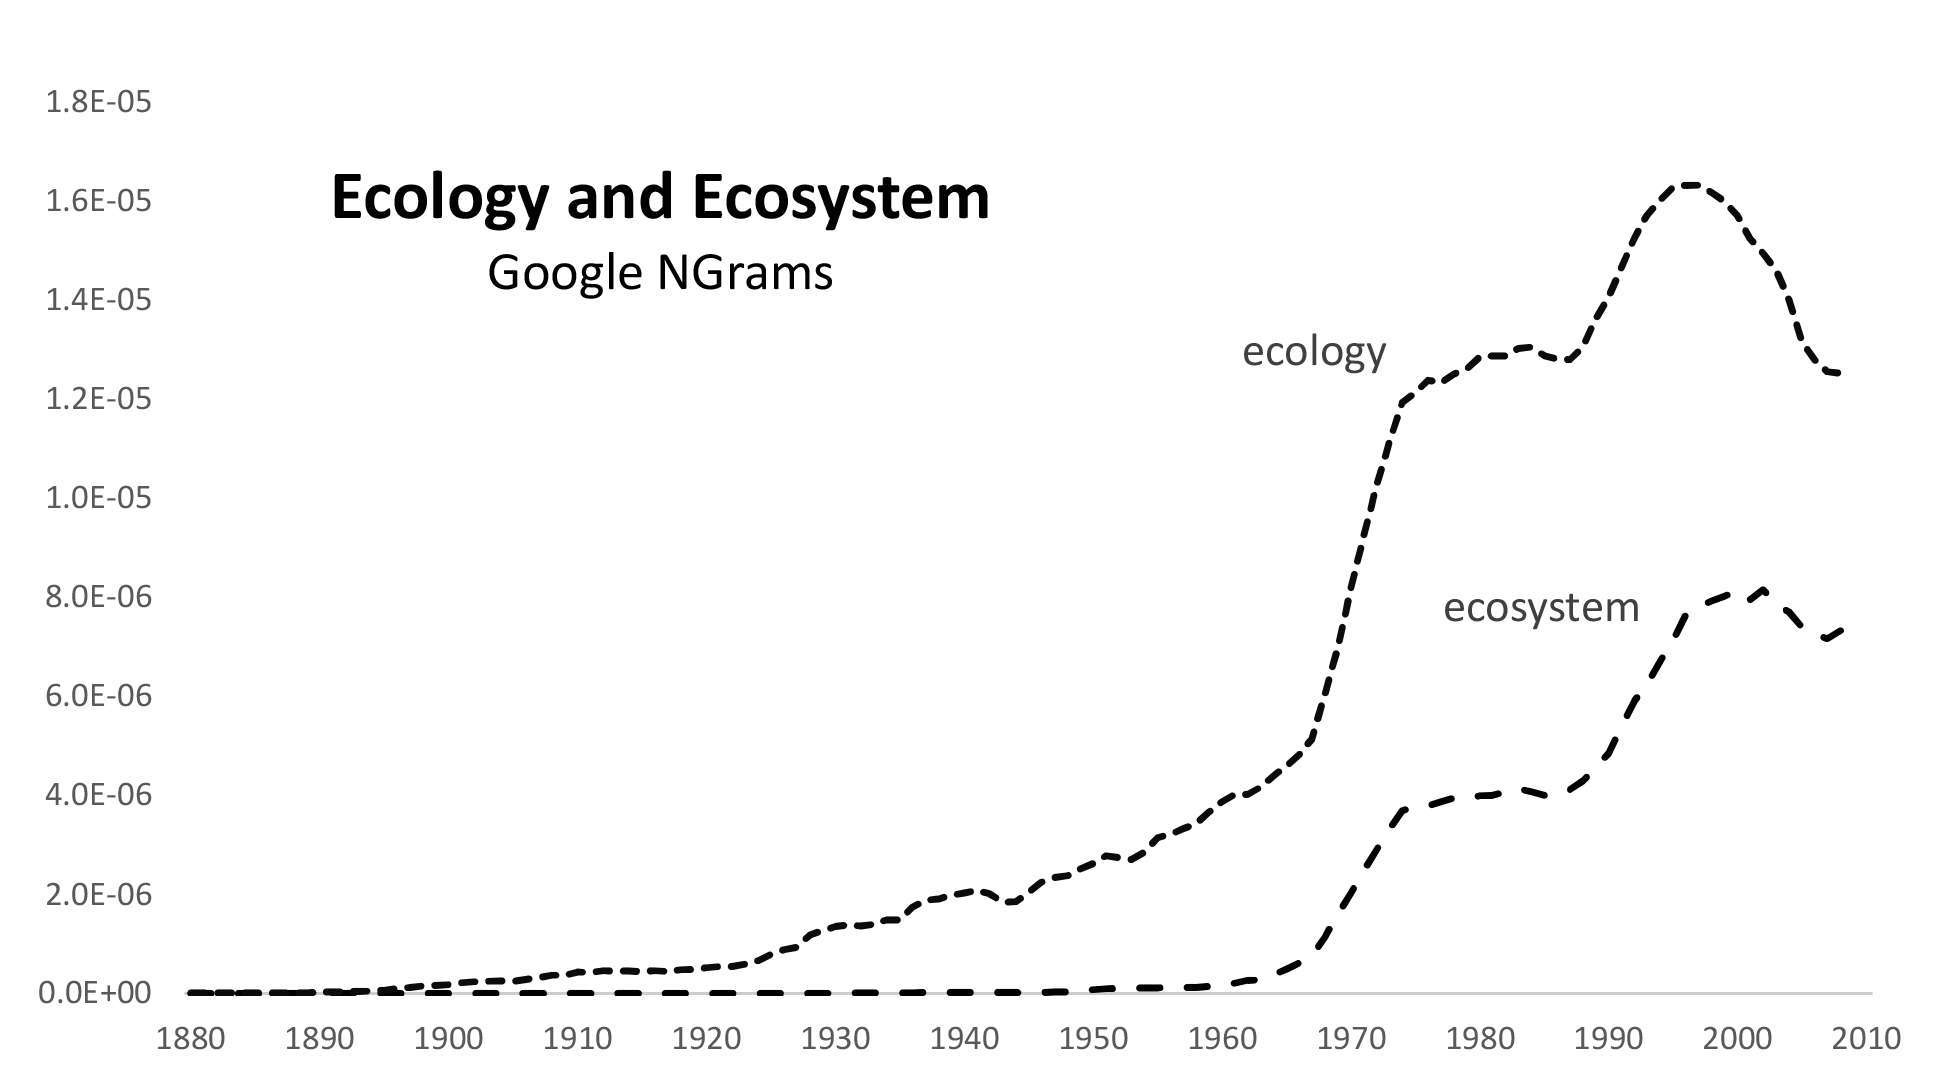
\includegraphics[width=5.5in]{figures/ecologyEcosystem}
  \caption{The emergent use of the words "ecology" and "ecosystem" as a Google Ngram. Note the first rapid rise in the 1970s generally attributable to the birth of the environmental movement sparked by Rachael Carson and the first Earth Day celebrated on April 22 1970. The second rise in the 1990s is harder to explain; perhaps the broad use of ecological metaphors outside of ecology?}
\end{figure}
 
 As writers, they were also fundamental in promoting two key principals in the environmental movement. First, that man is a part of nature and not outside of or above natural law. Leopold stated clearly that "The land ethic . . . simply enlarges the boundaries of the [human] community to include soils, waters, plants, and animals, or collectively the land" \citep[][p. 204{leopold_1949}. This reminds us that we cannot \textit{create} an ecosystem but we can be active participants in a community of living organisms with relationships between each other and  with non-living material flows. It is important to remember that, though perhaps a fish tank is an ecosystem created by humans, we do not define the rules of the system and instead we manage the system through an understanding of natures given laws. As Glacken observes, we have been doing this for a long time.

 And second, that there may be planetary limits to economic growth. There is still much debate that stems from Ehrlich's and Commoner's originally conceived arguments that presented opposing viewpoints. Of interest to our project is that one of the key pieces of literature, the Club of Rome Report or \textit{The Limits to Growth}, is based on a computer model of population and resources at a planetary scale. It represents another early intersection of data on population and natural resources, computational models, and global ecology \citep{meadows_1972}.
 
 The science of ecology is now a cornerstone of environmental management, conservation biology and sustainable resource management. Indeed much of the conservation management literature draws from ecological concepts and over the last several decades ecologists have promoted the idea of "adaptive management" to improve both social and environmental outcomes if conservation interventions \citep{holling_1978, leopold_1963}. As an alternative to long-term planning, adaptive management iterates planning, action, evaluation and modification as an ongoing process to accommodate shifting environmental and social factors. While one emphasis is on the constant iterative process, an equally important emphasis is on bringing people back into the sustainable management of ecosystems \citep{berkes_2000,holling_2002}. This is another place where the information ecosystem metaphor resonates powerfully with ecological thinking. Are there "information ecologists" who are key actors in the sustainable management of digital resources? Could these people be considered keystone species in an information ecosystem?